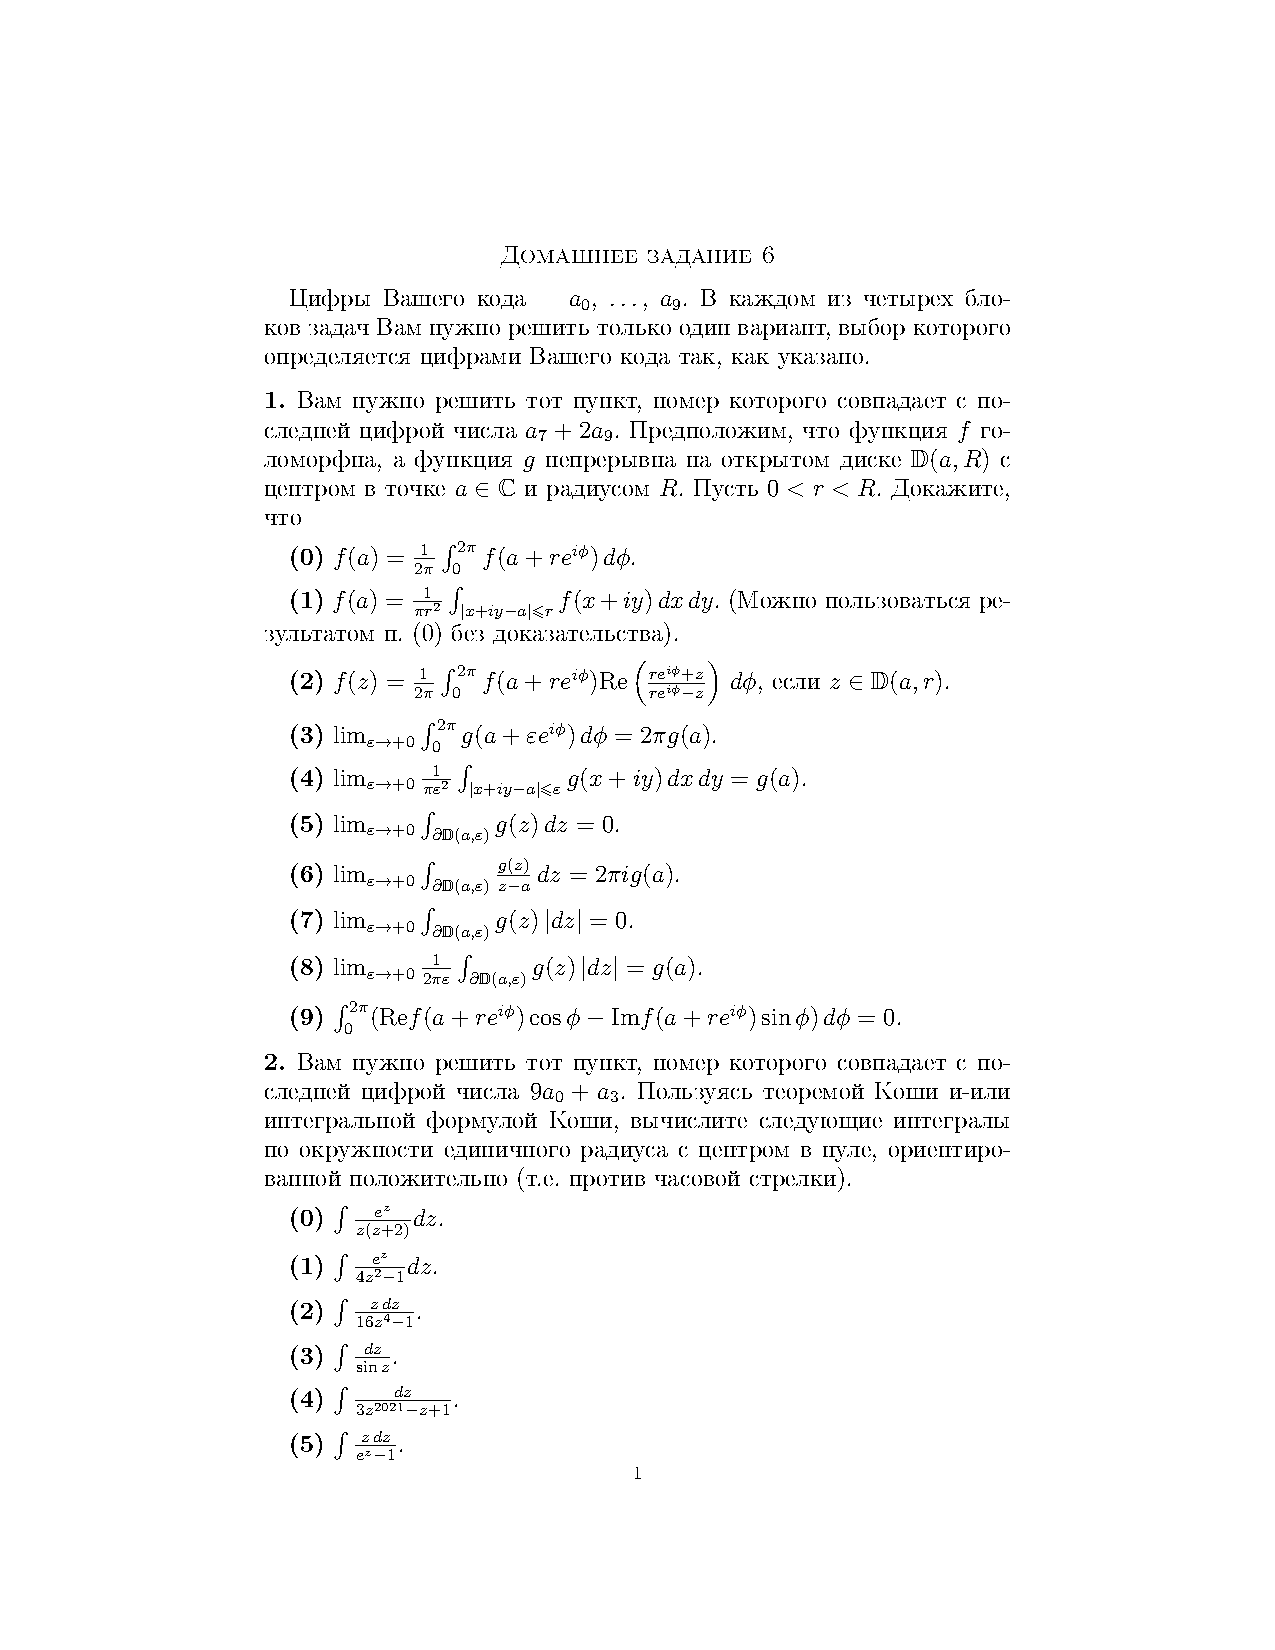
\includepdf[scale=1,pages=1-3]{Tasks/hw6}
\newpage
\section*{Решения}
\subsection*{Задача 1}
	Необходимо решить задачу $a_7 + 2a_9 = 3 + 2 \cdot 6 = 5 \mod 10$
	\begin{gather*}
		\lim\limits_{\varepsilon \to +0} \int_{\partial \mathbb{D} (a,\varepsilon)} g(z)dz = 0
	\end{gather*}
	Параметризуем окружность
	$z(\varphi) = a + \varepsilon e^{i \varphi},\ 0 \leqslant \varphi < 2\pi$
	Тогда
	\begin{gather*}
		\int_{\gamma} dz = \int_{A}^{B} |\gamma'(t)|dt\\
		dz
		= d(a + \varepsilon e^{i \varphi})
		= \varepsilon d e^{i \varphi}
		= \varepsilon i e^{i \varphi} d \varphi\\
	\end{gather*}
	Известно, что $g: \gamma \to \mathbb{C}$ -- непрерывная функция, тогда
	\begin{gather*}
		\lim\limits_{\varepsilon \to +0} \int_{\partial \mathbb{D} (a, \varepsilon)} g(z) dz
		= \lim\limits_{\varepsilon \to +0} \int_{\partial \mathbb{D} (a, \varepsilon)} g(a) \varepsilon i e^{i \varphi} d \varphi 
		= \lim\limits_{\varepsilon \to +0} \varepsilon\int_{\partial \mathbb{D} (a, \varepsilon)} g(a)i e^{i \varphi} d \varphi
		= 0
	\end{gather*}
\vskip 0.4in

\subsection*{Задача 2}
	Необходимо решить задачу $9a_0 + a_3 = 9 \cdot 1 + 9 = 8 \mod 10$
	\begin{gather*}
	\int \frac{dz}{4z^2 + 1}
	= \int \left(\frac{i}{2(2x+i)} - \frac{i}{2(2x - i)} \right)dz\\
	= \frac{1}{2}i \int \frac{1}{2z + i}dz - \frac{1}{2}i \int \frac{1}{2z - i} dz\\
	= \frac{1}{4}i \int \frac{1}{z + \frac{i}{2}}dz - \frac{1}{4}i \int \frac{1}{z - \frac{i}{2}} dz
	\end{gather*}
	Вопсользуемся интегральной формулой Коши
	\begin{gather*}
		1 = \frac{1}{2\pi i} \int \frac{1}{z + \frac{i}{2}} dz\qquad
		2\pi i = 2\pi i f(\frac{i}{2}) = \int \frac{1}{z + \frac{i}{2}}dz\\
		1 = \frac{1}{2\pi i} \int \frac{1}{z - \frac{i}{2}} dz\qquad
		2\pi i = 2\pi i f(-\frac{i}{2}) = \int \frac{1}{z - \frac{i}{2}}dz
	\end{gather*}
	Тогда
	\begin{gather*}
		\frac{1}{4}i \int \frac{1}{z + \frac{i}{2}}dz - \frac{1}{4}i \int \frac{1}{z - \frac{i}{2}} dz
		= \frac{1}{4}i \cdot 2 \pi i - \frac{1}{4}i \cdot 2 \pi i
		= 0
	\end{gather*}
\vskip 0.4in

\subsection*{Задача 3}
	Необходимо решить задачу $a_6 + 4a_8 = 9 + 4 \cdot 8 = 1 \mod 10$
	\begin{gather*}
		f(z) = \frac{e^z - 1}{z},\ a = 0\\
		e^z = \sum\limits_{n = 0}^{\infty} \frac{z^n}{n!}\\
		\frac{e^z}{z}
		= \sum\limits_{n = 0}^{\infty} \frac{z^{(n-1)}}{n!}\\
		\frac{e^z-1}{z}
		= \frac{e^z}{z} - \frac{1}{z}
		= \sum\limits_{n = 0}^{\infty} \frac{z^{(n-1)}}{n!} - \frac{1}{z}
		= \sum\limits_{n = 1}^{\infty} \frac{z^{(n-1)}}{n!}\\
	\end{gather*}
	Найдем радиус сходимости
	\begin{gather*}
		\sum\limits_{n = 1}^{\infty} \frac{z^{(n-1)}}{n!}\\
		R = \frac{1}{\overline{\lim\limits_{n \to \infty}}\sqrt[n]{\frac{1}{(n+1)!}}}
		= \overline{\lim\limits_{n \to \infty}}\sqrt[n]{(n+1)!} = \infty
	\end{gather*}
	\begin{comment}
		u_n = \frac{z^{(n-1)}}{n!}\\
		\left| \frac{u_{n+1}}{u_n}\right|
		= \left| \frac{\frac{z^{n}}{(n+1)!}}{\frac{z^{(n-1)}}{n!}} \right|
		= \left| \frac{z^n}{(n+1)z^{n-1}}\right|
		= \left| \frac{z}{(n+1)} \right|
		= \frac{|z|}{(n+1)} < 1\\
		|z| < 2
	\end{comment}
\vskip 0.4in

\subsection*{Задача 4}
	Необходимо решить задачу $a_1 + a_6 = 7 + 9 = 6 \mod 10$
	\begin{gather*}
		f(z) = \cos(\cos(\sin(z)))\\
		f(z) = \cos\left(\cos\left(z - \frac{z^3}{3!} + \frac{z^5}{5!} - \ldots\right)\right)
		= \cos\left(1 - \frac{\left(z - \frac{z^3}{3!} + \ldots\right)^2}{2!} + \frac{\left(z - \frac{z^3}{3!} + \ldots\right)^4}{4!} - \ldots\right)\\
		= 1 - \frac{\left(1 - \frac{\left(z - \frac{z^3}{3!} + \ldots\right)^2}{2!} + \ldots\right)^2}{2!} + \frac{\left(1 - \frac{\left(z - \frac{z^3}{3!} + \ldots\right)^2}{2!} + \ldots\right)^4}{4!} - \ldots
	\end{gather*}
	Заметим, что при раскрытии скобочек все полученные степени будут четными, а следовательно все нечетные производные будут равняться $0$, так как не будет ни одного элемента, не являющегося степенью $z$, а так как мы смотрим $z = 0$, то и $f^{(2n + 1)}(0)$ будет $0$.
\begin{comment}
		f(0) = \cos(\cos(\sin(0))) = \cos(1)\\
		f^{(1)}(0) = (\cos(\cos(\sin(0))))' = \sin(\sin(0))\cos(0)\sin(\cos(\sin(0))) = 0\\
		f^{(2)}(0) = \sin(1)\\
		f^{(3)}(0) = 0
\end{comment}